\documentclass[12pt]{article}
\usepackage{tikz}
\usepackage{pgfplots}
\pgfplotsset{compat=1.13}

\usepackage{extsizes}
\usepackage{caption}
\usepackage{multirow}

\usepackage{geometry} % Простой способ задавать поля
\geometry{top=30mm}
\geometry{bottom=30mm}
\geometry{left=25mm}
\geometry{right=20mm}

\usepackage[T2A]{fontenc}			% кодировка
\usepackage[utf8]{inputenc}	
\usepackage[english,russian]{babel}   %% загружает пакет многоязыковой вёрстки
\usepackage{indentfirst}

\usepackage{amsmath,amsfonts,amssymb,amsthm,mathtools} 
\usepackage{graphicx}
\begin{document}
	\begin{minipage}{0.45\linewidth}
	Работу выполнил\\
	Самохин Валентин, 676 гр.\\[2mm]
	под руководством\\
	Артанова А.\,А\,.
	\end{minipage}
	\hfill
	\begin{minipage}{0.45\linewidth}\flushright
		Маршрут~IX \ №~6\\[3mm]
		21~апреля 2017~г.,\\
		\end{minipage}
		
		\vspace{8mm}
		\begin{center}
			\textbf{\Large Лабораторная работа №~2.1.3:}\\[\parskip]
			\LARGE Определение $C_p/C_v$ по скорости звука в газе
			\end{center}
			\vspace{0mm}
			
			\paragraph{Цель работы:}
			\begin{enumerate}
				\item измерение частоты колебаний и длины волны при резонансе звуковых колебаний в газе, заполняющем трубу;
				\item определение показателя адиабаты с помощью уравнения состояния идеального газа.
			\end{enumerate}
			
			\paragraph{В работе используются:}
			звуковой генератор ГЗ; электронный
			осциллограф ЭО; микрофон; телефон; раздвижная труба; тепло
			изолированная труба, обогреваемая водой из термостата; баллон
			со сжатым углекислым газом; газгольдер.
			
			
			\vspace{2\parskip}
		\paragraph{Теоретическая справка.}
			Скорость распространения звуковой волны в газах зависит от показателя адиабаты $\gamma$. На измерении скорости звука основан один из наиболее точных методов определения показателя адиабаты.
			
			
			Скорость звука в газах определяется формулой:
			\begin{equation}\label{eq:speed}
			c=\sqrt{\gamma\dfrac{RT}{\mu}}.			
			\end{equation}
			
			Преобразуя формулу \ref{eq:speed}, найдем
			\begin{equation}\label{eq:speed2}
			\gamma=\dfrac{\mu}{RT}c^2.			
			\end{equation}
			
			Таким образом, для определения показателя адиабаты достаточно измерить температуру газа
			и скорость распространения звука (молярная масса газа предполагается известной). 
			
			Звуковая волна, распространяющаяся вдоль трубы, испытывает многократные отражения от торцов.
			Если длина трубы $L$ равна целому числу полуволн $L=n\lambda/2$, то волна, отраженная от торца трубы, вернувшаяся к ее началу и вновь отраженная, совпадает по фазе с падающей. Совпадающие по фазе волны усиливают друг друга. Амплитуда звуковых	колебаний при этом резко возрастает	— наступает \textit{резонанс}.  		
			
			При звуковых колебаниях слои газа, прилегающие к торцам трубы, не испытывают смещения (\textit{узел смещения}). Узлы смещения повторяются по всей длине трубы через $\lambda/2$. Между узлами находятcя
			максимумы смещения (\textit{пучности}).
			
			Скорость звука c связана с его частотой $f$ и длиной волны $\lambda$ соотношением
			\begin{equation}\label{eq:c}
				c=\lambda f.
			\end{equation}
			
			\paragraph{Методы измерений.}Подбор условий, при которых возникает резонанс, можно производить двояко:
			\begin{enumerate}
				\item При неизменной частоте $f$ и, как следствие, длины звуковой волны $\lambda$ можно \textbf{изменять длину трубы $L$}. Для этого применяется \textit{раздвижная труба}. Длина раздвижной трубы постепенно увеличивается, и наблюдается ряд последовательных резонансов. Возникновение резонанса легко наблюдать на осциллографе по резкому увеличению амплитуды
				колебаний. Для последовательных резонансов имеем
				\begin{eqnarray}
				L_n=n\dfrac{\lambda}{2}, & 	L_{n+1}=(n+1)\dfrac{\lambda}{2}, &L_{n+k} = n\dfrac{\lambda}{2} + k\dfrac{\lambda}{2},
				\end{eqnarray}	
				т. е. $\lambda/2$ равно \textit{угловому коэффициенту графика, изображающего зависимость длины трубы
				$L$ от номера резонанса	$k$}. Скорость звука	находится по формуле \ref{eq:c}.
				\item При постоянной длине трубы можно \textbf{изменять частоту звуковых
				колебаний}. В этом случае следует плавно \textit{изменять частоту $f$
				звукового генератора}, а следовательно, и длину звуковой волны $\lambda$. Для последовательных резонансов получим
				\begin{equation}\label{eq:way2}
					L=\dfrac{\lambda_1}{2}n=\dfrac{\lambda_2}{2}(n+1)=\dots=\dfrac{\lambda_{k+1}}{2}(n+k).
				\end{equation}	
				
				Из уравнений \ref{eq:c} и \ref{eq:way2} имеем
				\begin{equation*}
					f_1=\dfrac{c}{\lambda_1} = \dfrac{c}{2L}n, \ \ f_2=\dfrac{c}{2L}(n+1)=f_1 + \dfrac{c}{2L}
				\end{equation*}
				\begin{equation}
					f_{k+1} = \dfrac{c}{\lambda_{k+1}} = \dfrac{c}{2L}(n+k)=f_1+\dfrac{c}{2L}k.
				\end{equation}
	
			Таким образом, скорость звука, деленная на $2L$, определяется по \textit{угловому коэффициенту графика зависимости частоты от номера резонанса}.
		\end{enumerate}.
		\paragraph{Экспериментальная установка\\}
		Соответственно двум методам измерения скорости звука в работе имеются две установки. В обеих установках звуковые колебания в трубе возбуждаются \textbf{телефоном Т} и улавливаются \textbf{микрофоном М}. Мембрана телефона приводится в движение переменным током звуковой частоты; в качестве источника переменной ЭДС используется \textbf{звуковой генератор ЗГ} (генератор электрических колебаний звуковой и ультразвуковой частоты). Возникающий в микрофоне сигнал наблюдается на \textbf{осциллографе ЭО}.
	
	
		Микрофон и телефон присоединены к установке через тонкие резиновые трубки. Такая связь достаточна для возбуждения и обнаружения звуковых колебаний в трубе и в то же время мало возмущает эти колебания: при расчётах оба торца трубы можно считать неподвижными, а влиянием соединительных отверстий
		пренебречь. Первая установка (рис. \ref{pic1}) содержит раздвижную трубу с миллиметровой шкалой. Через патрубок (на рисунке не показан) труба может наполняться воздухом или углекислым газом из газгольдера. На этой установке производятся измерения $\gamma$ для воздуха и для $CO_2$. Вторая установка (рис. \ref{pic2}) содержит теплоизолированную трубу постоянной длины. Воздух в трубе нагревается водой из термостата. Температура газа принимается равной температуре воды, омывающей трубу. На этой установке измеряется зависимость скорости звука от температуры.


		\begin{figure}[h!]
			\begin{center}				
			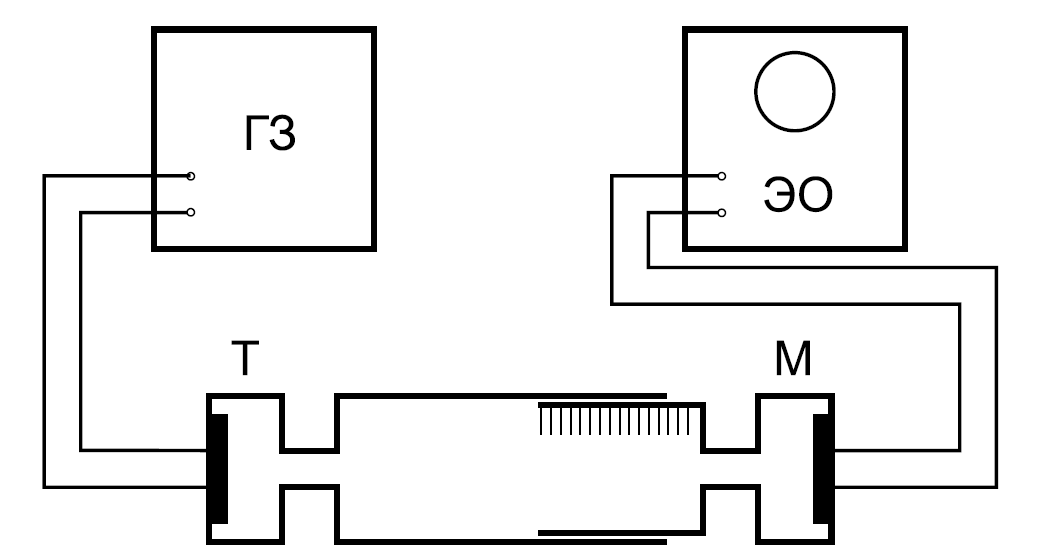
\includegraphics[width=0.75\textwidth]{pic1}
		\end{center}
			\caption{Установка для измерения скорости звука при помощи раздвижной трубы}\label{pic1}

		\end{figure}
	
		\begin{figure}[h!]
			\begin{center}
			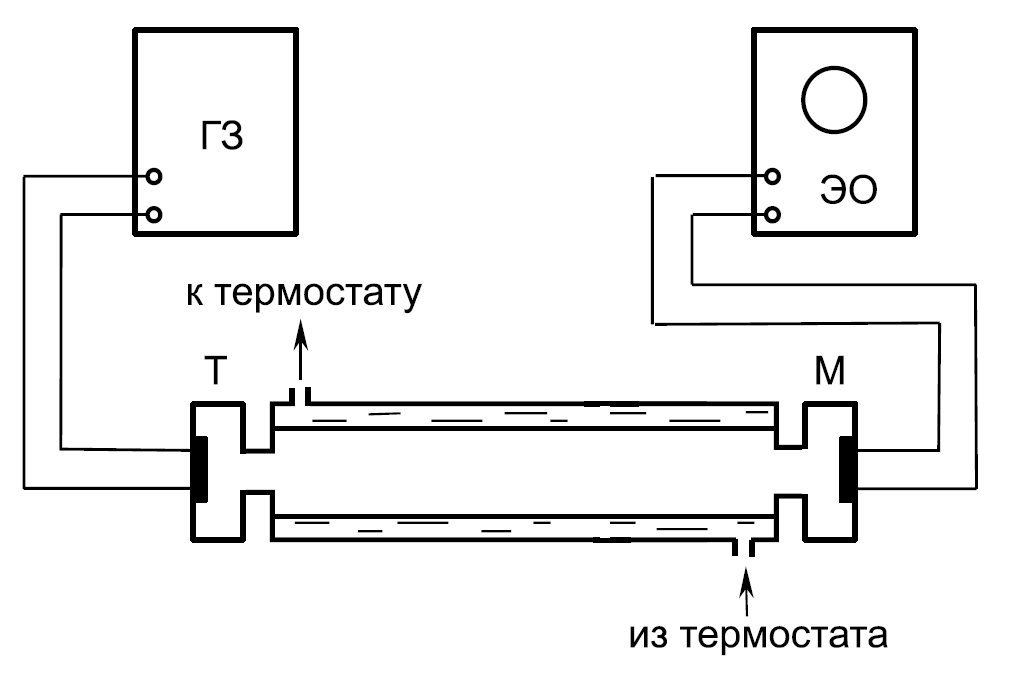
\includegraphics[width=0.75\textwidth]{pic2}
			\caption{Установка для изучения зависимости скорости звука от температуры}\label{pic2}
		\end{center}
		\end{figure}
		
		\clearpage
		\newpage
		\section*{Выполнение работы}
		Работа состояла из двух частей. На первой установке мы находили частоту резонанса при неизменной длине трубке сначала для воздуха, а затем для углекислого газа. На второй установке мы находили частоту резонанса при неизменной длине трубке для разных температур воздуха, нагревая его с помощью термостата.
		
		\subsection*{Измерения на первой установке}
		
		Открыв отверстие трубы, продули трубу воздухом. Закрыли отверстие. Предварительно рассчитав приблизительную частоту резонансов, начали их искать, постепенно увеличивая частоту генератора. Увеличение амплитуды устанавливали с помощью осциллографа. Затем уменьшая частоту генератора, убедились в неизменности результатов.
		%\noindent 
%		\Large\begin{tabular}{|c|c|c|c|c|c|c|c|}
%			\hline 
%	\multicolumn{2}{|l|}{Частота:}&\multicolumn{2}{|l|}{Частота:}&\multicolumn{2}{|l|}{Частота:}&\multicolumn{2}{|l|}{Частота:} \\ 
%			\hline 
%			№ & Удлинение & № & Удлинение & № & Удлинение & № & Удлинение \\ 
%			\hline 
%			& & & & & & & \\ 
%			\hline 
%			\hline 
%			& & & & & & & \\ 
%			\hline 
%			& & & & & & & \\ 
%			\hline 
%			& & & & & & & \\ 
%			\hline 
%			& & & & & & & \\ 
%			\hline 
%		\end{tabular}\captionof{table}{Измерение скорости звука в воздухе}
%		
%		\vspace{1cm}
%		\Large\begin{tabular}{|c|c|c|c|c|c|c|c|}
%			\hline 
%			\multicolumn{2}{|l|}{Частота:}&\multicolumn{2}{|l|}{Частота:}&\multicolumn{2}{|l|}{Частота:}&\multicolumn{2}{|l|}{Частота:} \\ 
%			\hline 
%			№ & Удлинение & № & Удлинение & № & Удлинение & № & Удлинение \\ 
%			\hline 
%			& & & & & & & \\ 
%			\hline 
%			& & & & & & & \\ 
%			\hline 
%			& & & & & & & \\ 
%			\hline 
%			& & & & & & & \\ 
%			\hline 
%			& & & & & & & \\ 
%			\hline 
%			& & & & & & & \\ 
%			\hline 
%		\end{tabular}\captionof{table}{Измерение скорости звука в $CO_2$}
		
%		\vspace{1cm}
		\noindent
	\begin{table}[h]

		\begin{center}
			\begin{tabular}{|c|c|c|c|}
			\hline
			\multicolumn{4}{|c|}{$L = 795\ mm$} \\
			\hline
			\multicolumn{2}{|c|}{Возрастание $f$} & \multicolumn{2}{|c|}{Убывание\ \ \    $f$}\\
			\hline
			№ & Частота $f$, \textit{Гц} & № & Частота $f$, \textit{Гц} \\
			\hline
			1& 225&1 &\multirow{5}{*}{Значения совпали}\\
			\cline{1-3}
			2& 480&2 &\\
			\cline{1-3}
			3& 655&3 &\\
			\cline{1-3}
			4& 865&4 &\\
			\cline{1-3}
			5& 1075&5 &\\
			\hline
		\end{tabular}
		\caption{Измерение частоты резонанса при постоянной длине трубки (воздух)}
	\end{center}
	\end{table}	
	
	
	\begin{minipage}{0.6\textwidth}
		\begin{tikzpicture}
		\begin{axis}[ xlabel={№ резонанса},ylabel={$f, \textit{Гц}$}, ymin = 160, ymax = 1150, xmin = 0.6, xmax = 5.3, grid = both ]
		\addplot [color=black, only marks] table[col sep = semicolon, y error index = 2] {plot1air.csv};
		\addplot [color=black, dashed] {208.5*x + 34.5};
		\end{axis}
		\end{tikzpicture}
		\captionof{figure}{График зависимости частоты от номера резонанса (опыт с воздухом)}
	\end{minipage}
	\vspace{0.05\textwidth}
	\begin{minipage}{0.25\textwidth}
		\centering
		$y = 208,5 x + 34.5$\\
		$\sigma_f = 2\ \textit{Гц}$\\
		$\frac{c}{2L} = (208,5 \pm 0,5)\  c^{-1}$\\
		$ c = (331,5 \pm 0,8)\ \textit{м/c}$\\
		
		
	\end{minipage}	
	
	Повторили действия, заменив воздух углекислым газом.
	
	\noindent
	\begin{table}[h]
		\begin{center}
		\begin{tabular}{|c|c|c|c|}
			\hline
			\multicolumn{4}{|c|}{$L = 795\ mm$} \\
			\hline
			\multicolumn{2}{|c|}{Возрастание $f$} & \multicolumn{2}{|c|}{Убывание\ \ \    $f$}\\
			\hline
			№ & Частота $f$, \textit{Гц} & № & Частота $f$, \textit{Гц} \\
			\hline
			1& 176&1 &\multirow{5}{*}{Значения совпали}\\
			\cline{1-3}
			2& 315&2 &\\
			\cline{1-3}
			3& 510&3 &\\
			\cline{1-3}
			4& 677&4 &\\
			\cline{1-3}
			5& 840&5 &\\
			\hline
		\end{tabular}
		\caption{Измерение частоты резонанса при постоянной длине трубки ($CO_2$)}
	\end{center}
		\end{table}
		
	 \begin{minipage}{0.6\textwidth}
	 \begin{tikzpicture}

	 \begin{axis}[ xlabel={№ резонанса},ylabel={$f, \textit{Гц}$}, ymin = 140, ymax = 900, xmin = 0.6, xmax = 5.3, grid = both]
	 \addplot [color=black, only marks] table[col sep = semicolon, y error index = 2] {plot1CO2.csv};
	 \addplot [color=black, dashed] {169*x - 3.4};
	 \end{axis}
	 \end{tikzpicture}
	 \centering\captionof{figure}{График зависимости частоты от номера резонанса (опыт с $CO_2$)}
	\end{minipage}
	\vspace{0.05\textwidth}
	\begin{minipage}{0.25\textwidth}
		\centering
		$y = 169 x - 3,4$\\
		$\sigma_f = 2\ \textit{Гц}$\\
		$\frac{c}{2L} = (169,0 \pm 0,3)\  c^{-1}$\\
		$ c = (268,7 \pm 0,5)\ \textit{м/c}$\\
		
		
	\end{minipage}
	
	Построив по полученным данным прямую, смогли установить значение $c/2L$ по коэффициенту наклона данной прямой, откуда несложно получить значение скорости воздуха.
	
	\subsection*{Измерения на второй установке}
	
	Измерим скорость воздуха при разных температурах. Для этого произведем измерения сначала при комнатной температуре, а затем с помощью термостата будем увеличивать температуру воздуха до 30, 40 и 50 градусов Цельсия. Действия такие же, как и при работе с первой установкой: увеличивая частоту генератора, будем искать резонансы.
	\begin{center}
	\begin{tabular}{|c|c|c|c|}
		\hline 
		\multicolumn{2}{|c|}{$T=22,9^{\circ} C$}&\multicolumn{2}{|c|}{$T=30^{\circ} C$}\\ 
		\hline 
		№ & Частота $f$, \textit{Гц} & № & Частота $f$, \textit{Гц}\\
		\hline 
		1&202 &1 &202 \\
		\hline 
		2&450 &2 & 455 \\ 
		\hline 
		3& 660&3 & 667 \\ 
		\hline 
		4&875 &4 & 884 \\ 
		\hline 
		5&1088 &5 & 1100 \\ 
		\hline 
		6&1302 &6 & 1319 \\ 
		\hline 
	\end{tabular}
\end{center}

\begin{minipage}{0.6\textwidth}
	\begin{tikzpicture}
	
	\begin{axis}[ xlabel={№ резонанса},ylabel={$f, \textit{Гц}$}, ymin = 160, ymax = 1380, xmin = 0.6, xmax = 6.3,  grid = both]
	\addplot [color=black, only marks] table[col sep = semicolon, y error index = 2] {plot2temp1.csv};
	\addplot [color=black, dashed] {217.97*x - 0.667};
	\end{axis}
	\end{tikzpicture}
	\centering\captionof{figure}{График зависимости частоты от номера резонанса ($T=22,9 ^{\circ} C$)}
\end{minipage}
\vspace{0.05\textwidth}
\begin{minipage}{0.25\textwidth}
	\centering
	$y = 217,97x - 0,667$\\
	$L = 800\ \textit{мм}$\\
	$\sigma_f = 2\ \textit{Гц}$\\
	$\frac{c}{2L} = (218,0 \pm 0,7)\  c^{-1}$\\
	$ c = (348,8 \pm 1,0)\ \textit{м/c}$\\
	
	
\end{minipage}

\begin{minipage}{0.6\textwidth}
	\begin{tikzpicture}
	
	\begin{axis}[ xlabel={№ резонанса},ylabel={$f, \textit{Гц}$}, ymin = 160, ymax = 1380, xmin = 0.6, xmax = 6.3,  grid = both]
	\addplot [color=black, only marks] table[col sep = semicolon, y error index = 2] {plot2temp2.csv};
	\addplot [color=black, dashed] {221.06*x - 2.533};
	\end{axis}
	\end{tikzpicture}
	\centering\captionof{figure}{График зависимости частоты от номера резонанса ($T=30 ^{\circ} C$)}
\end{minipage}
\vspace{0.05\textwidth}
\begin{minipage}{0.25\textwidth}
	\centering
	$y = 221,06 x - 2,533$\\
	$L = 800\ \textit{мм}$\\
	$\sigma_f = 2\ \textit{Гц}$\\
	$\frac{c}{2L} = (221,0 \pm 0,2)\  c^{-1}$\\
	$ c = (353,6 \pm 0,2)\ \textit{м/c}$\\
	
	
\end{minipage}


\begin{center}
	\begin{tabular}{|c|c|c|c|}
		\hline 
		\multicolumn{2}{|c|}{$T=40^{\circ} C$}& \multicolumn{2}{|c|}{$T=50^{\circ} C$}\\ 
		\hline 
		№ & Частота $f$, \textit{Гц} & № & Частота $f$, \textit{Гц} \\
		\hline 
		1&207 &1 &210  \\ 
		\hline 
		2&462 &2 &470  \\ 
		\hline 
		3&678 &3 &687  \\ 
		\hline 
		4&896 &4 &910 \\ 
		\hline 
		5&1118 &5 &1139  \\ 
		\hline 
		6&1334 &6 &1361 \\ 
		\hline 
	\end{tabular}\captionof{table}{Измерение частоты резонанса в воздухе при разных температурах}
\end{center}

\begin{minipage}{0.6\textwidth}
	\begin{tikzpicture}
	
	\begin{axis}[ xlabel={№ резонанса},ylabel={$f, \textit{Гц}$}, ymin = 160, ymax = 1400, xmin = 0.6, xmax = 6.3,  grid = both]
	\addplot [color=black, only marks] table[col sep = semicolon, y error index = 2] {plot2temp3.csv};
	\addplot [color=black, dashed] {223.46*x + 0.4};
	\end{axis}
	\end{tikzpicture}
	\centering\captionof{figure}{График зависимости частоты от номера резонанса ($T=40 ^{\circ} C$)}
\end{minipage}
\vspace{0.05\textwidth}
\begin{minipage}{0.25\textwidth}
	\centering
	$y =  223,46x + 0,4$\\
	$L = 800\ \textit{мм}$\\
	$\sigma_f = 2\ \textit{Гц}$\\
	$\frac{c}{2L} = (223,5 \pm 0,2)\  c^{-1}$\\
	$ c = (357,5 \pm 0,3)\ \textit{м/c}$\\
	
	
\end{minipage}
\\
\begin{minipage}{0.6\textwidth}
	\begin{tikzpicture}
	
	\begin{axis}[ xlabel={№ резонанса},ylabel={$f, \textit{Гц}$}, ymin = 160, ymax = 1400, xmin = 0.6, xmax = 6.3,  grid = both]
	\addplot [color=black, only marks] table[col sep = semicolon, y error index = 2] {plot2temp4.csv};
	\addplot [color=black, dashed] {228.14*x - 2.3333};
	\end{axis}
	\end{tikzpicture}
	\centering\captionof{figure}{График зависимости частоты от номера резонанса ($T=50 ^{\circ} C$)}
\end{minipage}
\vspace{0.05\textwidth}
\begin{minipage}{0.25\textwidth}
	\centering
	$y = 228.14 x - 2,33$\\
	$L = 800\ \textit{мм}$\\
	$\sigma_f = 2\ \textit{Гц}$\\
	$\frac{c}{2L} = (228,1 \pm 0,1)\  c^{-1}$\\
	$ c = (365,0 \pm 0,1)\ \textit{м/c}$\\	
	\end{minipage}
	
Построив по полученным данным прямую, смогли установить значение $c/2L$ по коэффициенту наклона данной прямой, откуда несложно получить значение скорости воздуха.

Для удобства, я совместил полученные значения скоростей звука в одной таблице, и там же привел полученные с помощью формулы \ref{eq:speed} значения показателя адиабаты.
\noindent
\begin{table}[h]

	\begin{tabular}{|c|c|c|c|c|c|c|}
		\hline
		&\multicolumn{2}{c|}{Опыт 1} & \multicolumn{4}{|c|}{Опыт 2}\\
		\hline
		&Воздух & $CO_2$ & $T=22,9 ^{\circ} C$ & $T=30 ^{\circ} C$ & $ T =40 ^{\circ} C$ & $T=50 ^{\circ} C$\\
		\hline
		с &$331,5 \pm 0,8$ & $268,7 \pm 0,5$ & $348,8 \pm 1,0$ & $353,6 \pm 0,2$ & $357,5 \pm 0,3$ & $365,0 \pm 0,1$\\
		\hline
		$\gamma$ & $1,32 \pm 0,01$ & $1,318 \pm 0,005$ & $1,43 \pm 0,01$ & $1,439 \pm 0,002$ & $ 1,424 \pm 0,003$ & $1,439 \pm 0,001$\\
		\hline 
		\end{tabular}
	\caption{Скорость звука c (\textit{м/с}) и показатель адиабаты $\gamma$ в разных опытах }
\end{table}

\section*{Вывод}
Мы измерили частоты колебаний при резонансе в газе и посчитали значения скорости звука и показателя адиабаты. Сравнивая результаты можно заметить, что:
\begin{enumerate}
	\item значения показателя адиабаты для воздуха (состоит преимущественно из двухатомных газов) колеблются около значения показателя адиабаты идеального двухатомного газа ($\gamma = 1,4$), но тем не менее, они не равны, что свидетельствует о том, что воздух не является идеальным газом, а также содержит недвухатомные газы.
	\item значения показателя адиабаты для углекислого газа также колеблются около значения показателя адиабаты идеального трехатомного газа ($\gamma = \frac{4}{3}$). Тем не менее, они отличаются, что также говорит о том, что углекислый газ не является идеальным газом.
	\item значения, полученные для воздуха в первом и втором опытах, отличаются. Предполагаю, что причина кроется в работе с первой установкой (негерметично закрывали отверстие или плохо продули воздухом и в трубе остался углекислый газ).
	\item[*] \textit{На лекции было сказано, что причина отличий кроется в том, что колебательные степени свободы молекул начинают вносить некоторый вклад в теплоемкость молекулы уже при температуре эксперимента.}
\end{enumerate}
\end{document}
